\subsection{Serial interfaces vs parallel interfaces}
\begin{itemize}
    \item Serial interfaces
        \begin{itemize}
            \item Encode bits by their temporal locations in the transmission medium
            \item Suitable for pin-limited devices
        \end{itemize}
    \item Parallel interfaces
    \begin{itemize}
        \item Encoded use spacial locality
    \end{itemize}
    \item Issues
    \begin{itemize}
        \item How does the device know when to start looking for information?
        \item What is the bit order?
        \item How does the receiver know when the transmission is complete?
    \end{itemize}
\end{itemize}

\subsection{Simplex, Full-Duplex and Half-Duplex}
\begin{figure}[H]
    \begin{center}
        \begin{circuitikz}
            % Simplex
            \draw node[buffer] (sim0) at (0, 0) {};
            \draw node[buffer] (sim1) at (4, 0) {};
            \draw (sim0.out) -- (sim1.in) node[above, midway, yshift=1cm] {{\large Simplex} {\small (One direction)}};
            \draw (sim0.in) -- ++(-1, 0);
            \draw (sim1.out) -- ++(1, 0);

            % Half Duplex
            \draw node[buffer] (hdup0) at (-1, -3) {};
            \draw node[buffer, rotate=180] (hdup1) at (-1, -4) {};

            \draw node[buffer] (hdup2) at (5, -3) {};
            \draw node[buffer, rotate=180] (hdup3) at (5, -4) {};

            \draw node[spdt, rotate=180] (sw0) at (1, -3.5) {};
            \draw node[spdt] (sw1) at (3, -3.5) {};

            \draw (hdup0.in) -- ++(-1, 0);
            \draw (hdup1.out) -- ++(-1, 0);
            \draw (hdup2.out) -- ++(1, 0);
            \draw (hdup3.in) -- ++(1, 0);

            \draw (hdup0.out) -| (sw0.out 2);
            \draw (hdup1.in) -| (sw0.out 1);
            \draw (hdup2.in) |- (sw1.out 1);
            \draw (hdup3.out) |- (sw1.out 2);

            \draw (sw0.in) -- (sw1.in) node[above, midway, yshift=1.25cm] {{\large Half Duplex} {\small (Both directions one at a time)}};

            % Full Duplex
            \draw node[buffer] (dup0) at (0, -7) {};
            \draw node[buffer] (dup1) at (4, -7) {};
            \draw (dup0.out) -- (dup1.in) node[above, midway, yshift=1cm] {{\large Full Duplex} {\small (Both directions simultaneously)}};
            \draw (dup0.in) -- ++(-1, 0);
            \draw (dup1.out) -- ++(1, 0);

            \draw node[buffer, rotate=180] (dup2) at (0, -8) {};
            \draw node[buffer, rotate=180] (dup3) at (4, -8) {};
            \draw (dup2.out) -- ++(-1, 0);
            \draw (dup3.in) -- ++(1, 0);
            \draw (dup2.in) -- (dup3.out);
        \end{circuitikz}
    \end{center}
    \caption{Simplex vs Full Duplex vs Half Duplex}
    \label{fig:sim-vs-duplex}
\end{figure}

\subsection{Asynchronous vs Synchronous}

\noindent \textbf{NOTE}: This is NOT required for analogue communications.

\begin{itemize}
    \item Asynchronous
    \begin{itemize}
        \item No clock signal transmitted
        \item Each end has a clock with the same \textit{nominal} frequency
        \item Clock and frame synchronization is required
    \end{itemize}
    \item Synchronous
    \begin{itemize}
        \item Clock is sent over a separate wire
        \item Clock signal is encoded within data (eg. Manchester Code)
    \end{itemize}
\end{itemize}

\subsection{Manchester Code}
With non-return to zero (NRZ) coding, clock synchronization would be difficult during long sequences
of either `1' of `0'. Manchester Code negates this by using the voltage transition to represent `1'
and `0'.
\begin{figure}[H]
    \begin{center}
        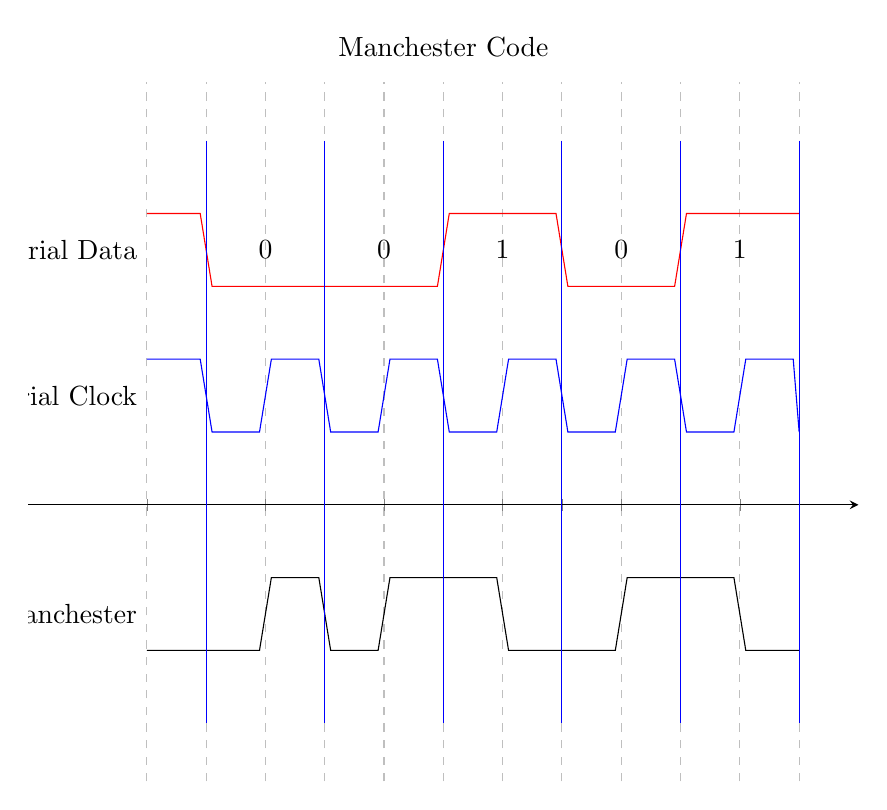
\begin{tikzpicture}
        \begin{axis} [
            width=\textwidth,
            axis x line=middle,
            axis y line=none,
            xmin=-20,
            xmax=120,
            xmajorgrids=true,
            grid style=dashed,
            xtick={0, 10, ..., 110},
            samples=1050,
            title=Manchester Code,
            xticklabels=\empty,
        ]
        
        % Serial Data
        \addplot[red] coordinates
        {(0,4) (9,4) (11,3) (49,3) (51,4) (69,4) (71,3) (89,3) (91,4) (110,4)};

        % Serial Clock
        \addplot[blue] coordinates
        {(0,2) (9,2) (11,1) (19,1) (21,2) (29,2) (31,1) (39,1) (41,2) (49,2) (51,1) (59,1) (61,2)
        (69,2) (71,1) (79,1) (81,2) (89,2) (91,1) (99, 1) (101, 2) (109,2) (110,1)};

        % Manchester
        \addplot[black] coordinates
        {(0,-2) (19,-2) (21,-1) (29,-1) (31,-2) (39,-2) (41,-1) (59,-1) (61,-2) (79,-2) (81,-1)
        (99,-1) (101,-2) (110,-2)};

        % Vertical Lines
        \addplot[blue] coordinates
        {(10,5) (10,-3)};
        \addplot[blue] coordinates
        {(30,5) (30,-3)};
        \addplot[blue] coordinates
        {(50,5) (50,-3)};
        \addplot[blue] coordinates
        {(70,5) (70,-3)};
        \addplot[blue] coordinates
        {(90,5) (90,-3)};
        \addplot[blue] coordinates
        {(110,5) (110,-3)};

        % Serial Data
        \node[] at (axis cs:20,3.5) {0};
        \node[] at (axis cs:40,3.5) {0};
        \node[] at (axis cs:60,3.5) {1};
        \node[] at (axis cs:80,3.5) {0};
        \node[] at (axis cs:100,3.5) {1};

        % Signal Labels
        \node[left] at (axis cs:0,3.5) {Serial Data};
        \node[left] at (axis cs:0,1.5) {Serial Clock};
        \node[left] at (axis cs:0,-1.5) {Manchester}; 
        \end{axis}
        \end{tikzpicture}
    \end{center}
    \caption{Manchester Code of `00101' serial data stream}
    \label{fig:manchester-code}
\end{figure}


\subsection{Serial Interface Comparison}
\begin{table}[H]
\caption{Technical comparison of different serial interfaces}
\label{table:serial-interface}
    \begin{center}
        \begin{tabular} { | m{4cm} | m{1cm} | m{1cm} | m{2.5cm} | m{1cm} | m{1cm} | m{1.5cm} | }
        \hline
        Interface & Sync. & Duplex & Wires & Mode & Topo. & Format\\
        \hline
        UART (RS232) & A & F & 2 + GND & SE & P & NRZ\\
        UART (RS423) & A & F & 2 + GND & SE & M & NRZ\\
        UART (RS422) & A & F & 4 + GND & D & M & NRZ\\
        UART (RS485) & A & F & 4 + GND & D & B & NRZ\\
        $\textrm{Synchronous}^{(1)}$ & S & F & 6 + GND & SE & P & NRZ\\
        SPI & S & F & 3 + GND & SE & M & NRZ\\
        JTAG & S & F & 4 + GND & SE & DC & NRZ\\
        I$^2$C/TWI & S & H & 2 + GND & SE & B & NRZ\\
        CAN & A & H & 2 + GND & D & B & NRZ-BS\\
        LIN & A & H & 1 + GND & S & B & NRZ\\
        Ethernet 100Base-T & S & F & $4$ & D & SH & MPE\\
        USB & A & H & 2 + GND/PWR & D & SH & NRZI-BS\\
        IEEE 1394 {\small (Firewire)} & S & F & 4 + GND/PWR & D & SH & DS\\
        Serial ATA & S & F & 4 + 3 GND & D & P & NRZ\\
        \hline
        \multicolumn{7}{l}{A = Asynchronous}\\
        \multicolumn{7}{l}{S = Synchronous}\\
        \multicolumn{7}{l}{F = Full duplex}\\
        \multicolumn{7}{l}{H = Half Duplex}\\
        \multicolumn{7}{l}{PWR = Power}\\
        \multicolumn{7}{l}{SE = Single ended {\small (Voltage signal with reference to ground)}}\\
        \multicolumn{7}{l}{D = Differential {\small (Complementary Signals)}}\\
        \multicolumn{7}{l}{P = Point to point}\\
        \multicolumn{7}{l}{M = Multipoint}\\
        \multicolumn{7}{l}{B = Bus}\\
        \multicolumn{7}{l}{DC = Daisy chain}\\
        \multicolumn{7}{l}{SH = Switch Hub}\\
        \multicolumn{7}{l}{NRZ = Non-return to zero}\\
        \multicolumn{7}{l}{NRZI = NRZ inverted}\\
        \multicolumn{7}{l}{DS = Data strobe}\\
        \end{tabular}
    \end{center}
\end{table}

\begin{table}[H]
    \caption{Application comparison of serial interfaces}
    \label{table:serial-app-comp}
    \begin{center}
        \begin{tabular} { | m{3cm} | m{2cm} | m{2cm} | m{2cm} | m{5cm} | }
        \hline
        Interface & Max \# Devices & Max Length (feet) & Max Speed (bps) & Application\\
        \hline
        USB (v1.0 \& v2.0) & 127 & 16 & 12M \& 480M & Human interface devices eg. mouse, keyboard\\
        \hline
        RS-232 & 2 & 50-100 & 20k & Modems/Terminals\\
        \hline
        RS-485 & 32 & 4000 & 10M & Data Acquisition, control systems\\
        \hline
        IrDA & 2 & 50-100 & 115k & Printers, hand-held computers\\
        \hline
        SPI & 8 & 10 & 2M [sic] $<$10M (device specific) & Microcontroller peripherals, EEPROM
        memory\\
        \hline
        $\textrm{I}^2\textrm{C}$ & 40 & 18 & 3.4M & As above\\
        \hline
        IEEE-1394 {\small (Firewire v(a) \& v(b))} & 64 & 15 & 400M, 800M & Video, mass storage
        systems\\
        \hline
        Ethernet & 1024 & 1600 & 10M / 100M / 1G / 2.5G / 5G / 10G / 100G & Networking\\
        \hline
        \end{tabular}
    \end{center}
\end{table}


\begin{figure}[H]
    \begin{center}
        \begin{tikzpicture}
            \node(top) [] {MCU Interfaces};
            \node(digital) [below of=top, yshift=-1cm, xshift=-4cm] {Digital};
            \node(analog) [below of=top, yshift=-1cm, xshift=4cm] {Analog};

            % Digital
            \node(on-off) [below of=digital, yshift=-1cm, xshift=-2cm] {On/Off};
            \node(parallel) [below of=digital, yshift=-1cm] {Parallel};
            \node(serial) [below of=digital, yshift=-1cm, xshift=2cm] {Serial};
            \node(async) [below of=serial, yshift=-1cm, xshift=-2cm] {Async.};
            \node(sync) [below of=serial, yshift=-1cm, xshift=2.5cm] {Sync.};
            \node(1wire) [align=left, below of=async, yshift=-0.25cm, xshift=2cm] {1-Wire};
            \node(rs232) [align=left, below of=1wire, yshift=-0.25cm] {RS232/RS485};
            \node(ethernet) [align=left, below of=rs232, yshift=-0.25cm] {Ethernet};
            \node(can) [align=left, below of=ethernet, yshift=-0.25cm] {CAN};
            \node(2wire) [below of=sync, yshift=-0.25cm, xshift=2.5cm] {2-Wire
            ($\textrm{I}^2\textrm{C}$)};
            \node(4wire) [below of=2wire, yshift=-0.25cm] {4-wire (SPI, Microwire)};
            \node(ssi) [below of=4wire, yshift=-0.25cm] {SSI};
            \node(jtag) [below of=ssi, yshift=-0.25cm] {JTAG};

            % Analog
            \node(voltage) [below of=analog, yshift=-1cm, xshift=-2cm] {Voltage};
            \node(current) [below of=analog, yshift=-1cm, xshift=2cm] {Current};

            % Draw Lines
            \draw (top) -- ++(0, -1) -| (digital) (top) ++(0, -1) -| (analog);
            \draw (digital) -- (parallel) (digital) ++(0, -1) -| (on-off) (digital) ++(0,-1) -|
            (serial);

            \draw (analog) -- ++(0, -1) -| (voltage) (analog) ++(0,-1) -| (current);

            \draw(serial) -- ++(0, -1) -| (async) (serial) ++(0, -1) -| (sync);
            \draw(async) |- (1wire);
            \draw(async) |- (rs232);
            \draw(async) |- (ethernet);
            \draw(async) |- (can);

            \draw(sync) |- (2wire);
            \draw(sync) |- (4wire);
            \draw(sync) |- (ssi);
            \draw(sync) |- (jtag);

        \end{tikzpicture}
    \end{center}
    \caption{Tree Chart of different interface types}
\end{figure}


\subsection{RS-232 vs RS-485}
\begin{table}[H]
    \begin{center}
        \begin{tabular} { | l | l | l | }
        \hline
        Parameter & RS-232 & RS-485\\
        \hline
        Line Configuration & Single Ended & Differential\\
        Mode of Operation & Simplex or full duplex & Simplex or half duplex\\
        Maximum cable length & 50 feet & 4000 feet\\
        Maximum data rate $^*$ & 20kbit/s & 10Mbit/s\\
        Typical logic levels & $\pm 5$ to $\pm 15$V & $\pm 1.5$ to $\pm 6$V\\
        Minimum receiver input impedance & 3 to 7k$\Omega$ & 12k$\Omega$\\
        Receiver sensitivity & $\pm 3$V & $\pm 200mV$\\
        \hline 
        \end{tabular}
    \end{center}
\end{table}


\subsection{SSI}
Synchronous Serial Interface (SSI) operates with a master slave model and is based off RS-422, is
point to point and used frame syncronization.

\begin{figure}[H]
\begin{center}
    \begin{circuitikz}
        \ctikzset{multipoles/thickness=3}
        \ctikzset{multipoles/dipchip/width=2}
        
        \draw (0,0) node[dipchip, num pins=6, hide numbers, no topmark, external pins
       width=0](txshift) {U0};
        \node[right] at (txshift.bpin 2) {\tiny CLK};
        \node[right] at (txshift.bpin 1) {\tiny Load};
        \draw (txshift.bpin 2) ++(0,0.1) -- ++(0.1,-0.1);
        \draw (txshift.bpin 2) ++(0,-0.1) -- ++(0.1,0.1);
        \node[left] at (txshift.bpin 6) {\tiny Q};


        \draw (5,0) node[dipchip, num pins=6, hide numbers, no topmark, external pins
       width=0](rxshift) {U1};
        \node[right] at (rxshift.bpin 1) {\tiny D};
        \node[right] at (rxshift.bpin 2) {\tiny CLK};
        \draw (rxshift.bpin 2) ++(0,0.1) -- ++(0.1,-0.1);
        \draw (rxshift.bpin 2) ++(0,-0.1) -- ++(0.1,0.1);
        \node[above] at (rxshift.s) {\tiny Rx Bus};
       
        \draw (5,-3) node[dipchip, num pins=6, hide numbers, no topmark, external pins
       width=0](rxdata) {U2};
        \node[right] at (rxdata.bpin 2) {\tiny CLK};
        \draw (rxdata.bpin 2) ++(0,0.1) -- ++(0.1,-0.1);
        \draw (rxdata.bpin 2) ++(0,-0.1) -- ++(0.1,0.1);
        \node[below] at (rxdata.n) {\tiny Rx in};
        
        \draw (5,-6) node[dipchip, num pins=6, hide numbers, no topmark, external pins
       width=0](rxframecounter) {U3};
        \node[right] at (rxframecounter.bpin 2) {\tiny CLK};
        \node[right] at (rxframecounter.bpin 1) {\tiny Clear};
        \draw (rxframecounter.bpin 2) ++(0,0.1) -- ++(0.1,-0.1);
        \draw (rxframecounter.bpin 2) ++(0,-0.1) -- ++(0.1,0.1);
        \node[left] at (rxframecounter.bpin 6) {\tiny DR};

        \draw (2, -3) node[buffer] (buf) {};

        % Draw Wires
        \draw (txshift.bpin 2) ++(-1,0) -- (txshift.bpin 2) ++(-0.5,0) node[circ]{} |- (buf.in)
        (txshift.bpin 2 |- 52, -3) ++(-0.25,0) node[crossing] {};

        \draw (txshift.bpin 1) -- ++(-1,0) (txshift.bpin 1) -- ++(-0.25, 0) node[circ]{} |- (rxframecounter.bpin 1); 

        \draw (buf.out) node[circ]{} |- (rxshift.bpin 2) (buf.out) |- (rxframecounter.bpin 2);

        \draw (txshift.bpin 1) ++(-1,0) node[left] {Tx Write};
        \draw (txshift.bpin 2) ++(-1,0) node[left] {CLK};

        \draw[line width=2pt] (txshift.n) -- ++(0,1) node[above] {Tx Data Bus};
        \draw (txshift.bpin 6) -- (rxshift.bpin 1) node[above, midway] {\tiny Serial data};

        \draw[line width=2pt] (rxshift.s) -- (rxdata.n);
        \draw[line width=2pt] (rxdata.s) |- ++(1.875, -0.3) node[right] {Rx Data Bus};
        \draw (rxframecounter.bpin 6) -- ++(1, 0) node[right]{Data Ready} ++(-0.3, 0) node[circ] {} |- (3, -4.5) |- (rxdata.bpin 2);

        \draw (0, -8) node[right] {DR=Data Ready} 
            ++(0, -0.5) node[right] {U0=Tx Shift Register}
            ++(0, -0.5) node[right] {U1=Rx Shift Register}
            ++(0, -0.5) node[right] {U2=Rx Data Register}
            ++(0, -0.5) node[right] {U3=Rx Frame Counter};
    \end{circuitikz}
\end{center}
\caption{Synchronous Serial Interface (SSI) Circuit}
\label{fig:ssi-circuit}
\end{figure}


A single SSI transmission is shown in Figure \ref{fig:ssi-wave}, to send multiple transmissions a
frame sync signal is sent on the LSB and the next transmission is sent.
\begin{figure}[H]
\begin{center}
    \begin{tikzpicture}
        \begin{axis}[
            width=0.8\textwidth,
            axis x line=middle,
            axis y line=none,
            xmajorgrids=true,
            grid style=dashed,
            xtick={0,10,...,120},
            xmin=-60,
            xmax=120,
            samples=1200,
            title=Synchronous Serial Interface,
            xticklabels=\empty,
        ]

        \addplot[red] coordinates
        {(-5,9) (-1,9) (1,11) (9,11) (11,9) (19,9) (21,11) (29,11) (31,9) (39,9) (41,11) (49,11)
        (51,9) (59,9) (61,11) (69,11) (71,9) (79,9) (81,11) (89,11) (91,9) (99,9) (101,11) (109,11)
        (111,9) (119,9)};

        \node[left] at (axis cs:-6,10) {CLK};
        \node[] at (axis cs:30,2) {MSB};
        \node[] at (axis cs:90,2) {LSB};

        \addplot[blue] coordinates
        {(-5,5) (-1,5) (1,7) (19,7) (21,5) (119,5)};
        
        \node[left] at (axis cs:-6,6) {Frame Sync};

        \addplot[black] coordinates
        {(-5,2) (20,2) (21,3) (39,3) (41,1) (59,1) (61,3) (79,3) (81,1) (99,1) (100,2) (119,2)};
        \addplot[black] coordinates
        {(20,2) (21,1) (39,1) (41,3) (59,3) (61,1) (79,1) (81,3) (99,3) (100,2)};
        
        \node[left] at (axis cs:-6,2) {Tx/Rx};
        \draw[darrow] (axis cs:20,1) -- (axis cs:100,1) node[midway,below] {4-16 bits};
        \end{axis}
    \end{tikzpicture}
\end{center}
\caption{Single SSI Trasmission}
\label{fig:ssi-wave}
\end{figure}


\subsection{SPI}
Serial Peripheral Interface (SPI), uses a master-slave model, is single ended, duplex, multipoint
and uses selection line based framing.

\begin{figure}[H]
\begin{center}
    \resizebox{\textwidth}{!}{
    \begin{circuitikz}
        \ctikzset{multipoles/thickness=3}
        \ctikzset{multipoles/dipchip/width=2}

        \draw (0,0) node[dipchip, num pins=6, hide numbers, no topmark, external pins
       width=0](msr) {MSR};
        \draw (msr.bpin 2) ++(0,0.1) -- ++(0.1,-0.1) -- ++(-0.1,-0.1);
        \draw (msr.bpin 1) node[right] {\tiny D}
            (msr.bpin 2) node[right] {\tiny CLK}
            (msr.bpin 3) node[right] {\tiny LOAD}
            (msr.bpin 6) node[left] {\tiny Q};
        \draw[line width=3pt] (-3,1.5) node[left] {Tx Data Bus} -| (msr.n);
        \draw[line width=3pt] (msr.s) |- (-3,-1.5) node[left] {Rx Data Bus};

        \draw (0,-5) node[dipchip, num pins=6, hide numbers, no topmark, external pins
       width=0](mfc) {MFC};
        \draw (mfc.bpin 2) ++(0,0.1) -- ++(0.1,-0.1) -- ++(-0.1,-0.1);
        \draw (mfc.bpin 1) node[right] {\tiny CNT} 
            (mfc.bpin 2) node[right] {\tiny CLK}
            (mfc.bpin 4) node[left] {\tiny RDY}
            (mfc.bpin 5) node[left] {\tiny SCK};
        
        \draw (8,0) node[dipchip, num pins=6, hide numbers, no topmark, external pins
       width=0](ssr) {SSR};
        \draw (ssr.bpin 2) ++(0,0.1) -- ++(0.1,-0.1) -- ++(-0.1,-0.1);
        \draw (ssr.bpin 1) node[right] {\tiny D}
            (ssr.bpin 2) node[right] {\tiny CLK}
            (ssr.bpin 6) node[left] {\tiny Q}
            (ssr.bpin 4) node[left] {\tiny LOAD};
        \draw[line width=2pt] (11, 1.5) node[right] {Tx Data Bus} -| (ssr.n);
        \draw[line width=2pt] (ssr.s) |- (11,-1.5) node[right] {Rx Data Bus};

        \draw (8,-5) node[dipchip, num pins=6, hide numbers, no topmark, external pins
       width=0](sfc) {SFC};
        \draw (sfc.bpin 2) ++(0,0.1) -- ++(0.1,-0.1) -- ++(-0.1,-0.1);
        \draw (sfc.bpin 2) node[right] {\tiny CLK}
            (sfc.bpin 6) node[left] {\tiny RDY};

        % Lines
        \draw (mfc) ++(5,0) node[buffer](buf){} (mfc.bpin 5) -- (buf.in) (buf.out) -- (sfc.bpin 2)
        ++(-0.5,0) node[circ]{} |- (ssr.bpin 2);
        \draw (mfc.bpin 5) ++(0.5,0) node[circ]{} |- (-2, -3.5) |- (msr.bpin 2);

        \draw (-3, 52 |- msr.bpin 3) node[left] {Tx Write} -- (msr.bpin 3)
            ++(-1, 0) node[circ]{} |- (mfc.bpin 1);

        \draw (-3, 52 |- mfc.bpin 2) node[left] {Clock} -- (mfc.bpin 2);
        \draw (mfc.bpin 4) -| (2,-6.5) -- (-3,-6.5) node[left] {Rx Ready};

        \draw (msr.bpin 6) -- (ssr.bpin 1);
        \draw (ssr.bpin 6) -| (10, 1.25) -- (-2, 1.25) |- (msr.bpin 1);
        
        \draw (ssr.bpin 4) -- (11, 52 |- ssr.bpin 4) node[right]{Tx Write};

        \draw (sfc.bpin 6) -- (11, 52 |- sfc.bpin 6) node[right]{Rx Ready};

        \draw (0,-6) node[right]{}
            ++(0,-0,5) node[right] {SSR=Slave Shift Register}
            ++(0,-0.5) node[right] {MSR=Master Shift Register}
            ++(0,-0.5) node[right] {MFC=Master Frame Counter}
            ++(0,-0.5) node[right] {SFC=Slave Frame Counter}
            ++(0,-0.5) node[right] {MOSI=Master out Slave in}
            ++(0,-0.5) node[right] {MISO=Master in Slave out}
            ++(0,-0.5) node[right] {SCK=Serial Clock};
    \end{circuitikz}
}
\end{center}
\caption{Circuit Diagram for SPI}
\label{fig:spi}
\end{figure}

SPI can be considered a simplified version of SSI, without frame synchronisation. The waveform for
the SPI protocol is shown in Figure \ref{fig:spi-wave}

\subsection{UART}
Universal Asynchronous Receive Transmit (UART) is a simple full duplex asynchronous serial
interface. UART has not framing beyond a single byte and required matched settings at both the
receiver and transmitter to avoid incorrect communications. UART has relatively high overheads and
can operate at most at 80\% efficiency. UART is also a free form protocol so can be adapted in
software to suit the application.

\begin{figure}[H]
\begin{center}
    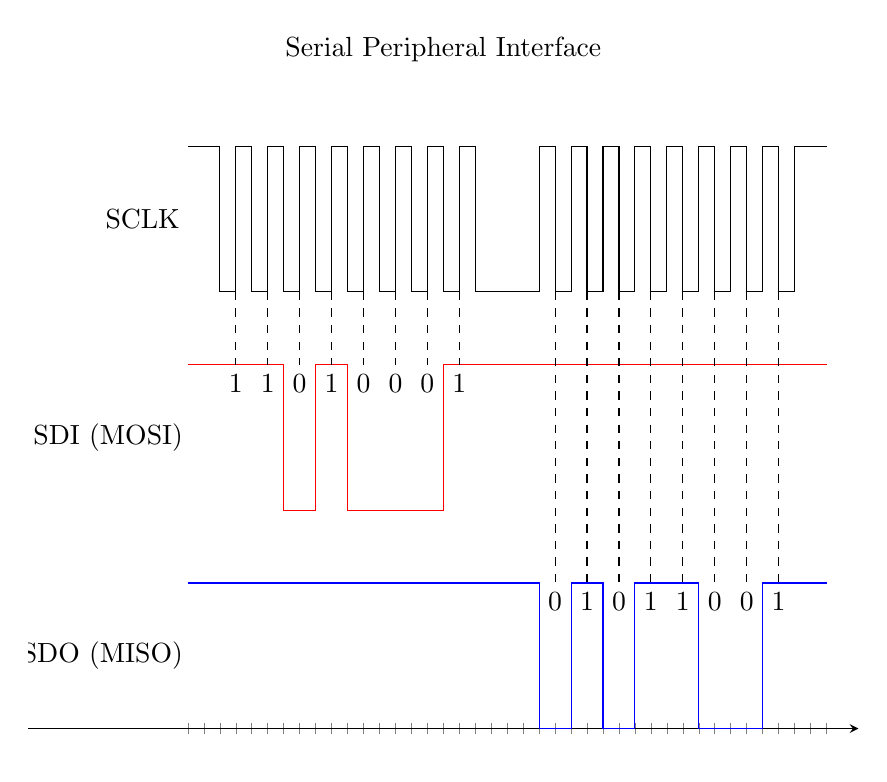
\begin{tikzpicture}
    \begin{axis}[
        width=\textwidth,
        axis x line=middle,
        axis y line=none,
        xmajorgrids=false,
        grid style=dashed,
        xtick={0,10,...,400},
        xmin=-100,
        xmax=420,
        samples=1000,
        title=Serial Peripheral Interface,
        xticklabels=\empty,
    ]
    % SCK
    \addplot[black] coordinates
    {(0,8) (20,8) (20,6) (30,6) (30,8) (40,8) (40,6) (50,6) (50,8) (60,8) (60,6) (70,6) (70,8)
    (80,8) (80,6) (90,6) (90,8) (100,8) (100,6) (110,6) (110,8) (120,8) (120,6) (130,6) (130,8) 
    (140,8) (140,6) (150,6) (150,8) (160,8) (160,6) (170,6) (170,8) (180,8) (180,6) (220,6) 
    (220,8) (230,8) (230,6) (240,6) (240,8) (250,8) (250,6) (260,6) (260,8) (270,8) (270,6)
    (280,6) (280,8) (290,8) (290,6) (300,6) (300,8) (310,8) (310,6) (320,6) (320,8) (330,8) (330,6) 
    (340,6) (340,8) (350,8) (350,6) (360,6) (360,8) (370,8) (370,6) (380,6) (380,8) (400,8)};
    
    % SDI (MOSI)
    \addplot[red] coordinates
    {(0,5) (60,5) (60,3) (80,3) (80,5) (100,5) (100,3) (160,3) (160,5) (400,5)};
    
    % SDO (MISO)
    \addplot[blue] coordinates
    {(0,2) (220,2) (220,0) (240,0) (240,2) (260,2) (260,0) (280,0) (280,2) (320,2) (320,0) (360,0)
    (360,2) (400,2)};

    % Draw Dashed Lines
    \draw[dashed] (axis cs:30,6) -- (axis cs:30,5) node[below] {1}
        (axis cs:50,6) -- (axis cs:50,5) node[below] {1}
        (axis cs:70,6) -- (axis cs:70,5) node[below] {0}
        (axis cs:90,6) -- (axis cs:90,5) node[below] {1}
        (axis cs:110,6) -- (axis cs:110,5) node[below] {0}
        (axis cs:130,6) -- (axis cs:130,5) node[below] {0}
        (axis cs:150,6) -- (axis cs:150,5) node[below] {0}
        (axis cs:170,6) -- (axis cs:170,5) node[below] {1};

    \draw[dashed] (axis cs:230,6) -- (axis cs:230,2) node[below] {0}
    (axis cs:250,6) -- (axis cs:250,2) node[below] {1}
    (axis cs:270,6) -- (axis cs:270,2) node[below] {0}
    (axis cs:290,6) -- (axis cs:290,2) node[below] {1}
    (axis cs:310,6) -- (axis cs:310,2) node[below] {1}
    (axis cs:330,6) -- (axis cs:330,2) node[below] {0}
    (axis cs:350,6) -- (axis cs:350,2) node[below] {0}
    (axis cs:370,6) -- (axis cs:370,2) node[below] {1};

    % Draw SDI, SCK etc.
    \draw (axis cs:1,7) node[left] {SCLK}
        (axis cs:3,4) node[left] {SDI (MOSI)}
        (axis cs:3,1) node[left] {SDO (MISO)};

    \end{axis}
    \end{tikzpicture}
\end{center}
\caption{SPI Transmission Waveform}
\label{fig:spi-wave}
\end{figure}


\subsection{I$^2$C/TWI}
Inter-integrated circuit (I$^2$C) or Two wire interface (TWI) is a simple, robust a d easy to use
communication system for use between a microcontroller and several external peripherals (bus type
protocol). I$^2$C is availible in standard speed at 100kbps, full-speed at 400kbps and high-speed
at 3.33Mbps. The bus supports up to 127 devices in parallel. The protocol is half duplex and
synchronous (\textit{More complicated than SPI with slave select}). This protocol is robust as every
byte has an ACK response to verify the receipt of the message, there is also built in arbitration to
eliminate bus conflicts using Carrier sense multiple access/collision detection.\\

\noindent The protocol uses 8-bit words and master slave handshaking where the master generates the clock
signal and initiates the communication. Within the transmission there is an address byte for device
selection, a read write bit for declaring reading and writing operations.\\

\subsubsection{Clock Stretching}
Clock stretching is when a slow slave device pulls the clock line low until it is ready to transmit
data, this allows the slower device to send at a usable rate for its application.

\begin{figure}[H]
\begin{center}
    \begin{tikzpicture}
        \node[xwboxes] (app) {Application};
        \node[xwboxes, below of=app] (pres) {Presentation};
        \node[xwboxes, below of=pres] (sess) {Session};
        \node[xwboxes, below of=sess] (tran) {Transport};
        \node[xwboxes, below of=tran] (net) {Network};
        \node[xwboxes, below of=net, fill=blue!8] (data) {Data Link $\frac{\textrm{Logical Link
        Control (LLC)}}{\textrm{Media Access Control (MAC)}}$};
        \node[xwboxes, below of=data, fill=gray!8] (phy) {Physical};

        % Label
        \draw[darrow] (data.north west) ++(-0.5,0)  -- ++(0,-2) node[left, midway] {I$^2$C/TWI};

        % Info
        \draw[dashed] (data.north east) -- (6, 2) node[right]{\textbf{Object Layer}}
            ++(0, -0.5) node[right] {Prioritiser message handling}
            ++(0,-0.5) node[right] {acceptance filtering}
            ++(0, -0.5) node[right] {\textbf{Transfer layer}}
            ++(0,-0.5) node[right] {Fault confinement}
            ++(0,-0.5) node[right] {Error detection}
            ++(0,-0.5) node[right] {Acknowledgment}
            ++(0,-0.5) node[right] {Message framing}
            ++(0,-0.5) node[right] {Arbitration} -- (data.south east);

        \draw[dashed] (phy.north east) -- (6,-3) node[right] {\textbf{Physical Layer}}
           ++(0,-0.5) node[right] {Bit representation} 
           ++(0,-0.5) node[right] {Transfer rate} 
           ++(0,-0.5) node[right] {Signal level and timing} 
           ++(0,-0.5) node[right] {Transmission medium} -- (phy.south east); 
    \end{tikzpicture}
\end{center}
\caption{OSI Protocol stack for I$^2$C/TWI}
\label{fig:i2c-osi}
\end{figure}


The process of a master to slave transmission is shown in Figure \ref{fig:i2c-master-slave}.

\begin{figure}[H]
\begin{center}
\begin{adjustbox} {height=0.9\textheight}
    \begin{tikzpicture}
        \draw (0,0) node[wwboxes] (0) {Set TWI clock (CKDIV) This is only needed once};
        \draw (0,-4) node[wwboxes] (1) {Set the control register -Master Enable \textit{TWI\_CR = MSEN}};
        \draw (0,-8) node[wwboxes] (2) {Set the master mode register -Device slave address (DAAR)
        -Transfer direction bit Write ==> bit MREAD=0};
        \draw (8,0) node[wwboxes] (3) {Load transmit register \textit{TWI\_THR} = Data to send};
        \draw (8,-4) node[wwboxes] (4) {Read status register};
        \draw (8,-8) node[wdiamond] (5) {\textit{TXRDY == 1} check};
        \draw (8,-12) node[wwboxes] (6) {Read status register};
        \draw (8,-16) node[wdiamond] (7) {\textit{TXCOMP == 1} check};
        
        % Draw Arrows
        \draw[arrow] (0,2) node[above] {Begin} -- (0.north);
        \draw[arrow] (0.south) -- (1.north);
        \draw[arrow] (1.south) -- (2.north);
        \draw (2.south) |- (4,-11);
        \draw (4,-11) -- (4,2);
        \draw[arrow] (4,2) -| (3.north);
        \draw[arrow] (3.south) -- (4.north);
        \draw[arrow] (4.south) -- (5.north);
        \draw[arrow] (5.south) -- (6.north);
        \draw[arrow] (6.south) -- (7.north);
        \draw[arrow] (7.south) -- (8,-20) node[below] {Finish};

        \draw[arrow] (5.east) -- (12,-8) |- (8,-2);
        \draw[arrow] (7.east) -- (12,-16) |- (8,-10.75);
    \end{tikzpicture}
\end{adjustbox}
\end{center}
\caption{Master to slave transfer process and signaling on I$^2$C}
\label{fig:i2c-master-slave}
\end{figure}


\subsubsection{I$^2$C Write}
To write to a slave the send the start condition and starts the clock then send the 7-bit slave
address with the MSB first. The master then send the `0' write bit the slave then responds with an
ACK (`0'). The master then sends data (This can be several bytes). The slave then sends an ACK (`0')
and finally the master sends the stop condition.

\subsubsection{I$^2$C Read}
To read from a slave the master sends the start condition then starts the clock. The 7-bit slave
address is then transmitted with MSB first. To indicate a read the master then sends a `1' read bit.
The selected slave then responds with a ACK (`0'). The slave then sends the appropriate bit stream
(This can be several bytes). The master finally responds with a NACK then the stop condition.\\ 

\noindent To complete a full read from an external sensor the master must frist perform a write
operation to the slave then perform a read.

\subsubsection{Packet Structure}
The packet structure of I$^2$C is shown in Figure \ref{fig:serial-packet}, This is for writing, to
preform a read operation the R/W bit is set to `1' to indicate a read and in the data byte a NACK is
used instead of the ACK (\textit{ACK=1, NACK=0}). 
\begin{figure}[H]
\begin{center}
    \begin{tikzpicture}
        \node[smboxes] (start) {Start};
        \node[xsmboxes, right of=start, xshift=1.5cm] (0) {};
        \node[xsmboxes, right of=0, xshift=0.75cm] (1) {};
        \node[xsmboxes, right of=1, xshift=0.75cm] (2) {};
        \node[xsmboxes, right of=2, xshift=0.75cm] (3) {};
        \node[xsmboxes, right of=3, xshift=0.75cm] (4) {};
        \node[xsmboxes, right of=4, xshift=0.75cm] (5) {};
        \node[xsmboxes, right of=5, xshift=0.75cm] (6) {};
        \node[xsmboxes, right of=6, xshift=0.75cm] (7) {\tiny RW};
        \node[xsmboxes, right of=7, xshift=0.75cm] (ACK) {\tiny ACK};
       
        
        \node[xsmboxes, below of=start, yshift=-2cm, xshift=1.5cm] (01) {};
        \node[xsmboxes, right of=01, xshift=0.75cm] (11) {};
        \node[xsmboxes, right of=11, xshift=0.75cm] (21) {};
        \node[xsmboxes, right of=21, xshift=0.75cm] (31) {};
        \node[xsmboxes, right of=31, xshift=0.75cm] (41) {};
        \node[xsmboxes, right of=41, xshift=0.75cm] (51) {};
        \node[xsmboxes, right of=51, xshift=0.75cm] (61) {};
        \node[xsmboxes, right of=61, xshift=0.75cm] (71) {};
        \node[xsmboxes, right of=71, xshift=0.75cm] (ACK1) {\tiny ACK};
        
        \node[xsmboxes, below of=01, yshift=-3cm] (02) {};
        \node[xsmboxes, right of=02, xshift=0.75cm] (12) {};
        \node[xsmboxes, right of=12, xshift=0.75cm] (22) {};
        \node[xsmboxes, right of=22, xshift=0.75cm] (32) {};
        \node[xsmboxes, right of=32, xshift=0.75cm] (42) {};
        \node[xsmboxes, right of=42, xshift=0.75cm] (52) {};
        \node[xsmboxes, right of=52, xshift=0.75cm] (62) {};
        \node[xsmboxes, right of=62, xshift=0.75cm] (72) {};
        \node[xsmboxes, right of=72, xshift=0.75cm] (ACK2) {\tiny ACK};
        \node[smboxes, right of=ACK2, xshift=1.5cm] (stop) {Stop};

        \draw (7.north east) ++(0,0.25) node[] (controlend) {};
        \draw (ACK.south west) ++(0,-0.25) node[] (ACKstart) {};
        \draw (71.north east) ++(0,0.25) node[] (addrend) {};
        \draw (ACK1.south west) ++(0,-0.25) node[] (ACK1start) {};
        \draw (02.south west) ++(0,-0.25) node[] (datastart) {};
        \draw (stop.north east) ++(0,0.25) node[] (stopend) {};
        \draw (ACK.south west) ++(0,-0.2) node[] (ACKstartlabel) {};
        \draw (ACK1.south west) ++(0,-0.2) node[] (ACK1startlabel) {};
        \draw (ACK2.north west) ++(0,0.2) node[] (ACK2startlabel) {};

        % Arrows
        \draw[arrow, blue] (start.north west) ++(0,0.25) -- (controlend);
        \draw[arrow, red] (ACK.south east) ++(0,-0.25) -- (ACKstart);
        \draw[arrow, blue] (01.north west) ++(0,0.25) -- (addrend);
        \draw[arrow, red] (ACK1.south east) ++(0,-0.25) -- (ACK1start);
        \draw[arrow, blue] (stop.north west) ++(0,0.25) -- (stopend);
        \draw[arrow, red] (ACK2.south east) ++(0,-0.25) -- (datastart);

        % Text Labels
        \draw (start) ++(-1,0) node[left] {\textbf{Control Byte}};
        \draw (01) ++(-1,0) node[left] {\textbf{Address Byte (MSB First)}};
        \draw (02) ++(-1,0) node[left] {\textbf{Data Byte (MSB First)}};

        % Byte Labels
        \draw[darrow] (0.south west) ++(0,-0.2) -- (ACKstartlabel) node[below,midway] {Slave Address};
        \draw[darrow] (01.south west) ++(0,-0.2) -- (ACK1startlabel) node[below,midway] {Memory
        Address};
        \draw[darrow] (02.north west) ++(0,0.2) -- (ACK2startlabel) node[above,midway] {Data
        Sample};

        % Key
        \draw[arrow,blue] (0,-6) -- ++(0.5, 0) node[right] {\textit{Master to Slave on SDA}};
        \draw[arrow,red] (0.5,-6.5) node[right] {\textit{Slave to Master on SDA}} -- ++(-0.5,0);

    \end{tikzpicture}
\end{center}
\caption{Serial Packet Structure}
\label{fig:serial-packet}
\end{figure}


\subsubsection{Multi-master Operation}
Multi-master operation is supported on I$^2$C however, in this mode arbitration is required as
several masters may attempt to control the bus simultaneously. For this to work every master in a
multi-master must be configured to a multi-master setup as single masters don't arbitrate, causing
interference if a single master is connected. The master device controls SDA and SCK.

Arbitration simply allows the faster (or slower) device to access the channel. To detect if the
channel is in use the SDA and SCL lines are checked to see if they are LOW.

\subsubsection{Collision Detection}
A collision is where more than one device is transmitting on the SDA line at once. To perform
collision detection a device has to be able to read the SDA line while checking the SDA for
transmitted bits. And if the two don't match then a collision has occurred. This is determined using
the XOR of the requested bit and the line data, shown in Figure \ref{fig:collision-detect}.

\begin{figure}[H]
\begin{center}
    \begin{circuitikz}[american]
        \node[xor port, rotate=-90] at (2, -2) (xor) {};
        \node[pmos] at (5, -1.25) (fet){};

        % Draw Lines
        \draw (0,0) -| (fet.source);
        \draw (0,0) -- (6,0) node[right] {SDA};
        \draw (fet.drain) -- ++(0,-0.5) node[ground]{};

        \draw (0,-0.5) -| (fet.gate);
        \draw(0,-0.5) -| (xor.in 2);
        \draw (0,0) -| (xor.in 1);
        \draw (xor.out) |- (0,-3) node[left] {Collision};

        \node[left] at (0,0) {RXD};
        \node[left] at (0,-0.5) {TXD};
    \end{circuitikz}
\end{center}
\caption{I$^2$C Collision Detection Circuitry}
\label{fig:collision-detect}
\end{figure}

